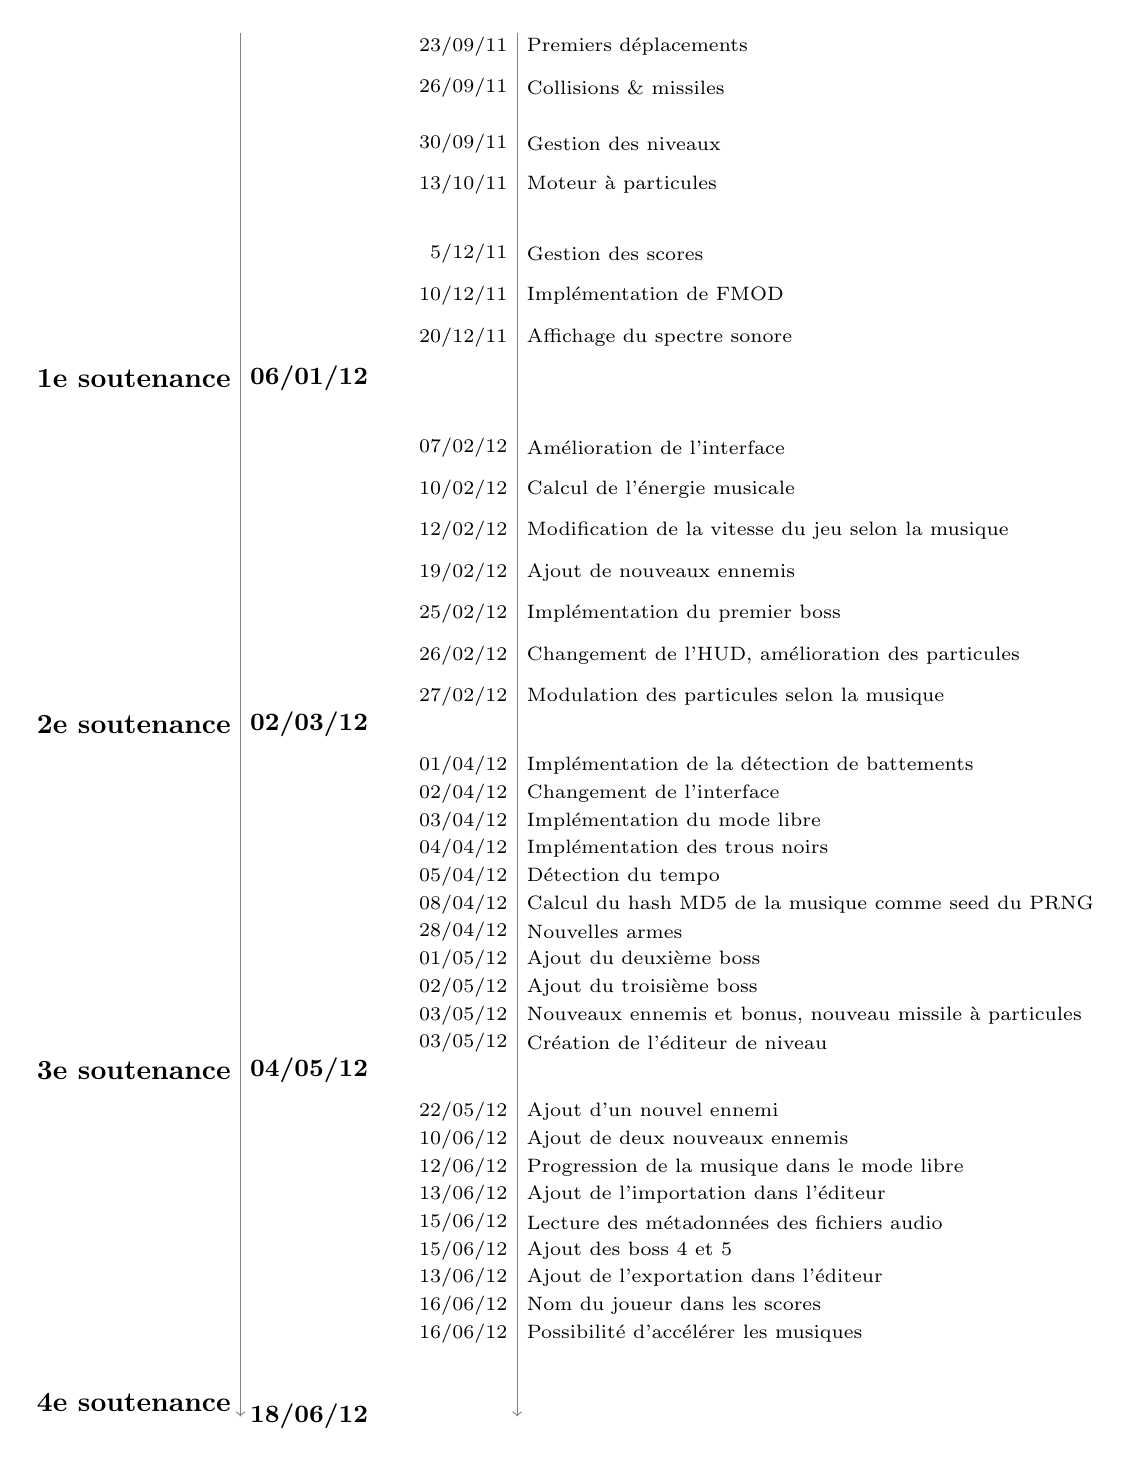
\begin{tikzpicture}
	\draw[gray,->] (0,0) coordinate (tl1start) -- ++(0,-500pt) coordinate
	(tl1end);
	\draw[gray,->] (tl1start)++(100pt,0) coordinate (tl2start)-- +
	+(0,-500pt) coordinate (tl2end);
	\path (tl1start) --
		node[left,pos=0.25] {\textbf{1e soutenance}}
		node[left,pos=0.50] {\textbf{2e soutenance}}
		node[left,pos=0.75] {\textbf{3e soutenance}}
		node[left,pos=0.99] {\textbf{4e soutenance}}
		node[right,pos=0.25] {\small{\textbf{06/01/12}}}
		node[right,pos=0.50] {\small{\textbf{02/03/12}}}
		node[right,pos=0.75] {\small{\textbf{04/05/12}}}
		node[right,pos=1] {\small{\textbf{18/06/12}}}
	(tl1end);
	\path (tl2start) --
	node[left,pos=0.01] {\scriptsize{23/09/11}}
	node[right,pos=0.01] {\scriptsize{Premiers déplacements}}
	node[left,pos=0.04] {\scriptsize{26/09/11}}
	node[right,pos=0.04] {\scriptsize{Collisions \& missiles}}
	node[left,pos=0.08] {\scriptsize{30/09/11}}
	node[right,pos=0.08] {\scriptsize{Gestion des niveaux}}
	node[left,pos=0.11] {\scriptsize{13/10/11}}
	node[right,pos=0.11] {\scriptsize{Moteur à particules}}
	node[left,pos=0.16] {\scriptsize{5/12/11}}
	node[right,pos=0.16] {\scriptsize{Gestion des scores}}
	node[left,pos=0.19] {\scriptsize{10/12/11}}
	node[right,pos=0.19] {\scriptsize{Implémentation de FMOD}}
	node[left,pos=0.22] {\scriptsize{20/12/11}}
	node[right,pos=0.22] {\scriptsize{Affichage du spectre sonore}}
	%Soutenance 1
	node[left,pos=0.30] {\scriptsize{07/02/12}}
	node[right,pos=0.30] {\scriptsize{Amélioration de l'interface}}
	node[left,pos=0.33] {\scriptsize{10/02/12}}
	node[right,pos=0.33] {\scriptsize{Calcul de l'énergie musicale}}
	node[left,pos=0.36] {\scriptsize{12/02/12}}
	node[right,pos=0.36] {\scriptsize{Modification de la vitesse du jeu selon la musique}}
	node[left,pos=0.39] {\scriptsize{19/02/12}}
	node[right,pos=0.39] {\scriptsize{Ajout de nouveaux ennemis}}
	node[left,pos=0.42] {\scriptsize{25/02/12}}
	node[right,pos=0.42] {\scriptsize{Implémentation du premier boss}}
	node[left,pos=0.45] {\scriptsize{26/02/12}}
	node[right,pos=0.45] {\scriptsize{Changement de l'HUD, amélioration des particules}}
	node[left,pos=0.48] {\scriptsize{27/02/12}}
	node[right,pos=0.48] {\scriptsize{Modulation des particules selon la musique}}
	%Soutenance 2
	node[left,pos=0.53] {\scriptsize{01/04/12}}
	node[right,pos=0.53] {\scriptsize{Implémentation de la détection de battements}}
	node[left,pos=0.55] {\scriptsize{02/04/12}}
	node[right,pos=0.55] {\scriptsize{Changement de l'interface}}
	node[left,pos=0.57] {\scriptsize{03/04/12}}
	node[right,pos=0.57] {\scriptsize{Implémentation du mode libre}}
	node[left,pos=0.59] {\scriptsize{04/04/12}}
	node[right,pos=0.59] {\scriptsize{Implémentation des trous noirs}}
	node[left,pos=0.61] {\scriptsize{05/04/12}}
	node[right,pos=0.61] {\scriptsize{Détection du tempo}}
	node[left,pos=0.63] {\scriptsize{08/04/12}}
	node[right,pos=0.63] {\scriptsize{Calcul du hash MD5 de la musique comme seed du PRNG}}
	node[left,pos=0.65] {\scriptsize{28/04/12}}
	node[right,pos=0.65] {\scriptsize{Nouvelles armes}}
	node[left,pos=0.67] {\scriptsize{01/05/12}}
	node[right,pos=0.67] {\scriptsize{Ajout du deuxième boss}}
	node[left,pos=0.69] {\scriptsize{02/05/12}}
	node[right,pos=0.69] {\scriptsize{Ajout du troisième boss}}
	node[left,pos=0.71] {\scriptsize{03/05/12}}
	node[right,pos=0.71] {\scriptsize{Nouveaux ennemis et bonus, nouveau missile à particules}}
	node[left,pos=0.73] {\scriptsize{03/05/12}}
	node[right,pos=0.73] {\scriptsize{Création de l'éditeur de niveau}}
	%Soutenance 3
	node[left,pos=0.78] {\scriptsize{22/05/12}}
	node[right,pos=0.78] {\scriptsize{Ajout d'un nouvel ennemi}}
	node[left,pos=0.80] {\scriptsize{10/06/12}}
	node[right,pos=0.80] {\scriptsize{Ajout de deux nouveaux ennemis}}
	node[left,pos=0.82] {\scriptsize{12/06/12}}
	node[right,pos=0.82] {\scriptsize{Progression de la musique dans le mode libre}}
	node[left,pos=0.84] {\scriptsize{13/06/12}}
	node[right,pos=0.84] {\scriptsize{Ajout de l'importation dans l'éditeur}}
	node[left,pos=0.86] {\scriptsize{15/06/12}}
	node[right,pos=0.86] {\scriptsize{Lecture des métadonnées des fichiers audio}}
	node[left,pos=0.88] {\scriptsize{15/06/12}}
	node[right,pos=0.88] {\scriptsize{Ajout des boss 4 et 5}}
	node[left,pos=0.90] {\scriptsize{13/06/12}}
	node[right,pos=0.90] {\scriptsize{Ajout de l'exportation dans l'éditeur}}
	node[left,pos=0.92] {\scriptsize{16/06/12}}
	node[right,pos=0.92] {\scriptsize{Nom du joueur dans les scores}}
	node[left,pos=0.94] {\scriptsize{16/06/12}}
	node[right,pos=0.94] {\scriptsize{Possibilité d'accélérer les musiques}}
	(tl2end);
\end{tikzpicture}

\par (Ceci n'est pas (seulement) un prétexte pour jouer avec tikzfig).